% \documentclass[dvipdfmx, 11pt]{beamer}
\documentclass[aspectratio=169, dvipdfmx, 11pt]{beamer} % aspectratio=43, 149, 169
\usepackage{here, amsmath, latexsym, amssymb, bm, ascmac, mathtools, multicol, tcolorbox, subfig}

%デザインの選択(省略可)
\usetheme{Luebeck}
%カラーテーマの選択(省略可)
\usecolortheme{orchid}
%フォントテーマの選択(省略可)
\usefonttheme{professionalfonts}
%フレーム内のテーマの選択(省略可)
\useinnertheme{circles}
%フレーム外側のテーマの選択(省略可)
\useoutertheme{infolines}
%しおりの文字化け解消
\usepackage{atbegshi}
\ifnum 42146=\euc"A4A2
\AtBeginShipoutFirst{\special{pdf:tounicode EUC-UCS2}}
\else
\AtBeginShipoutFirst{\special{pdf:tounicode 90ms-RKSJ-UCS2}}
\fi
%ナビゲーションバー非表示
\setbeamertemplate{navigation symbols}{}
%既定をゴシック体に
\renewcommand{\kanjifamilydefault}{\gtdefault}
%タイトル色
\setbeamercolor{title}{fg=structure, bg=}
%フレームタイトル色
\setbeamercolor{frametitle}{fg=structure, bg=}
%スライド番号のみ表示
%\setbeamertemplate{footline}[frame number]
%itemize
\setbeamertemplate{itemize item}{\small\raise0.5pt\hbox{$\bullet$}}
\setbeamertemplate{itemize subitem}{\tiny\raise1.5pt\hbox{$\blacktriangleright$}}
\setbeamertemplate{itemize subsubitem}{\tiny\raise1.5pt\hbox{$\bigstar$}}
% color
\newcommand{\red}[1]{\textcolor{red}{#1}}
\newcommand{\green}[1]{\textcolor{green!40!black}{#1}}
\newcommand{\blue}[1]{\textcolor{blue!80!black}{#1}}

\renewcommand{\figurename}{図}
\renewcommand{\tablename}{表}
\setbeamertemplate{caption}[numbered]

\title[研究紹介]{研究紹介}
\subtitle{〜凸解析と集合最適化〜}
\author[岩本 崚汰]{岩本 崚汰}
\institute[新潟大学大学院]{新潟大学大学院 自然科学研究科 数理科学専攻}
\date{\today}

\begin{document}
\maketitle

\begin{frame}{凸解析}
  R. Tyrrell Rockafellarによって1950年代に提唱された凸解析は, 凸集合や凸関数を中心に広く研究が進められている.
  \begin{block}{凸集合}
    集合$C$が凸集合であるとは,任意の$x, y\in C$と任意の$\lambda\in[0, 1]$に対して
    \[
      \lambda x + (1-\lambda)y\in C
    \]
    が成り立つことをいう.
  \end{block}
  \centering
  \begin{figure}
    \begin{minipage}{.45\textwidth}
      \centering
      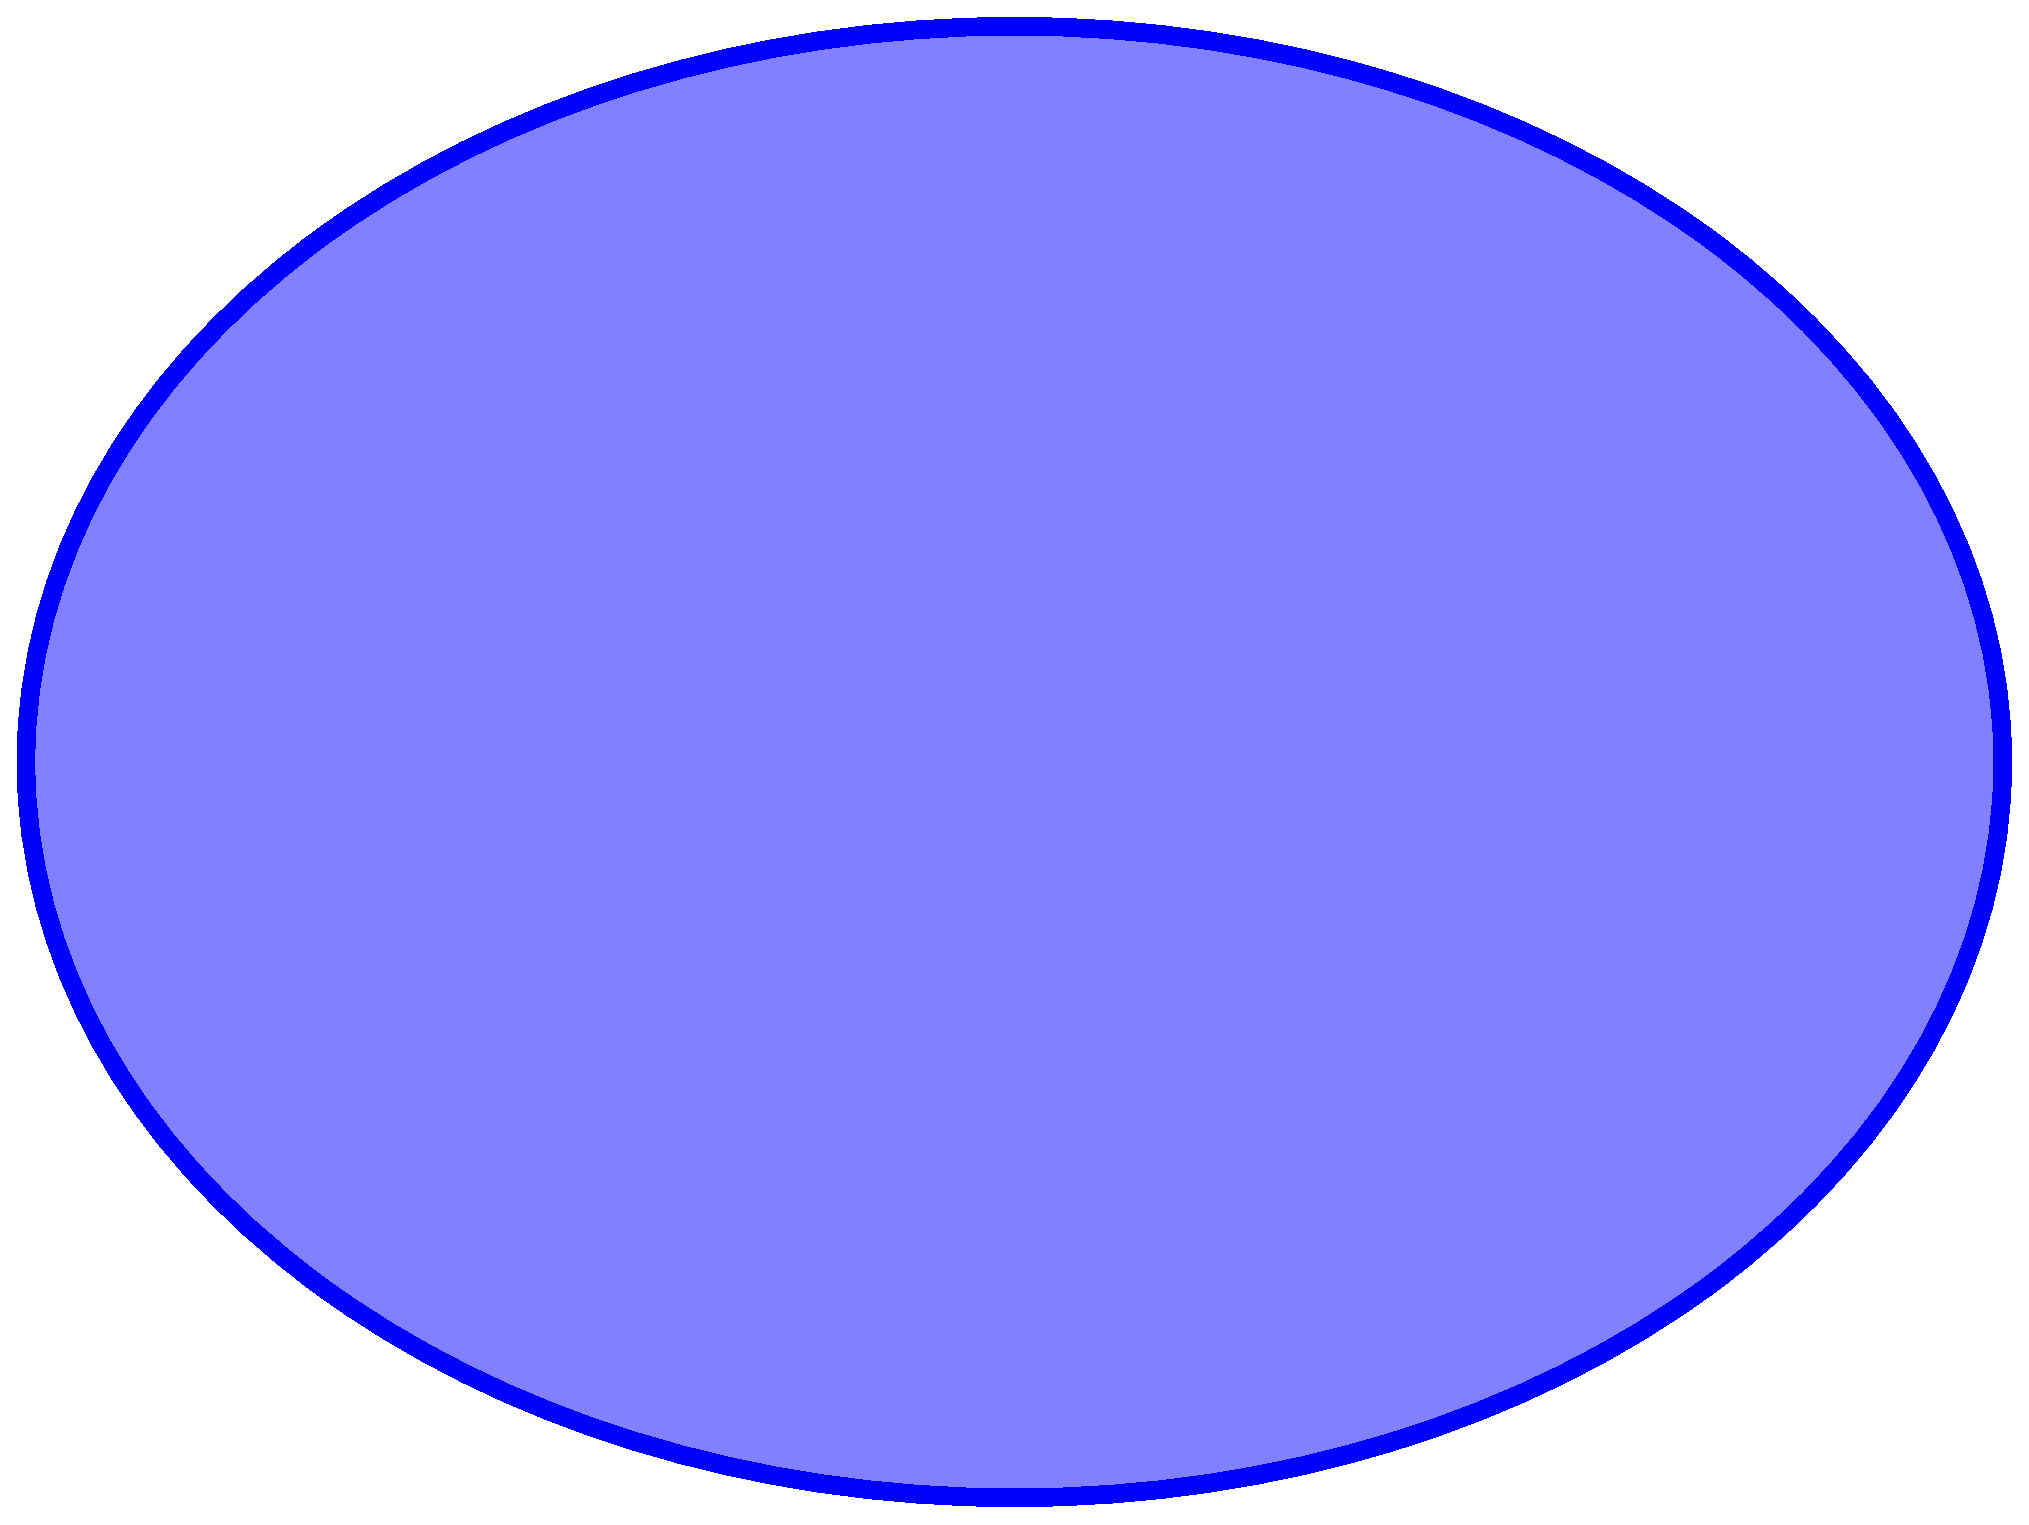
\includegraphics[keepaspectratio, scale=0.095]{figures/eps/convex_set.eps}
      \caption{凸集合}
    \end{minipage}\hfill
    \begin{minipage}{.45\textwidth}
      \centering
      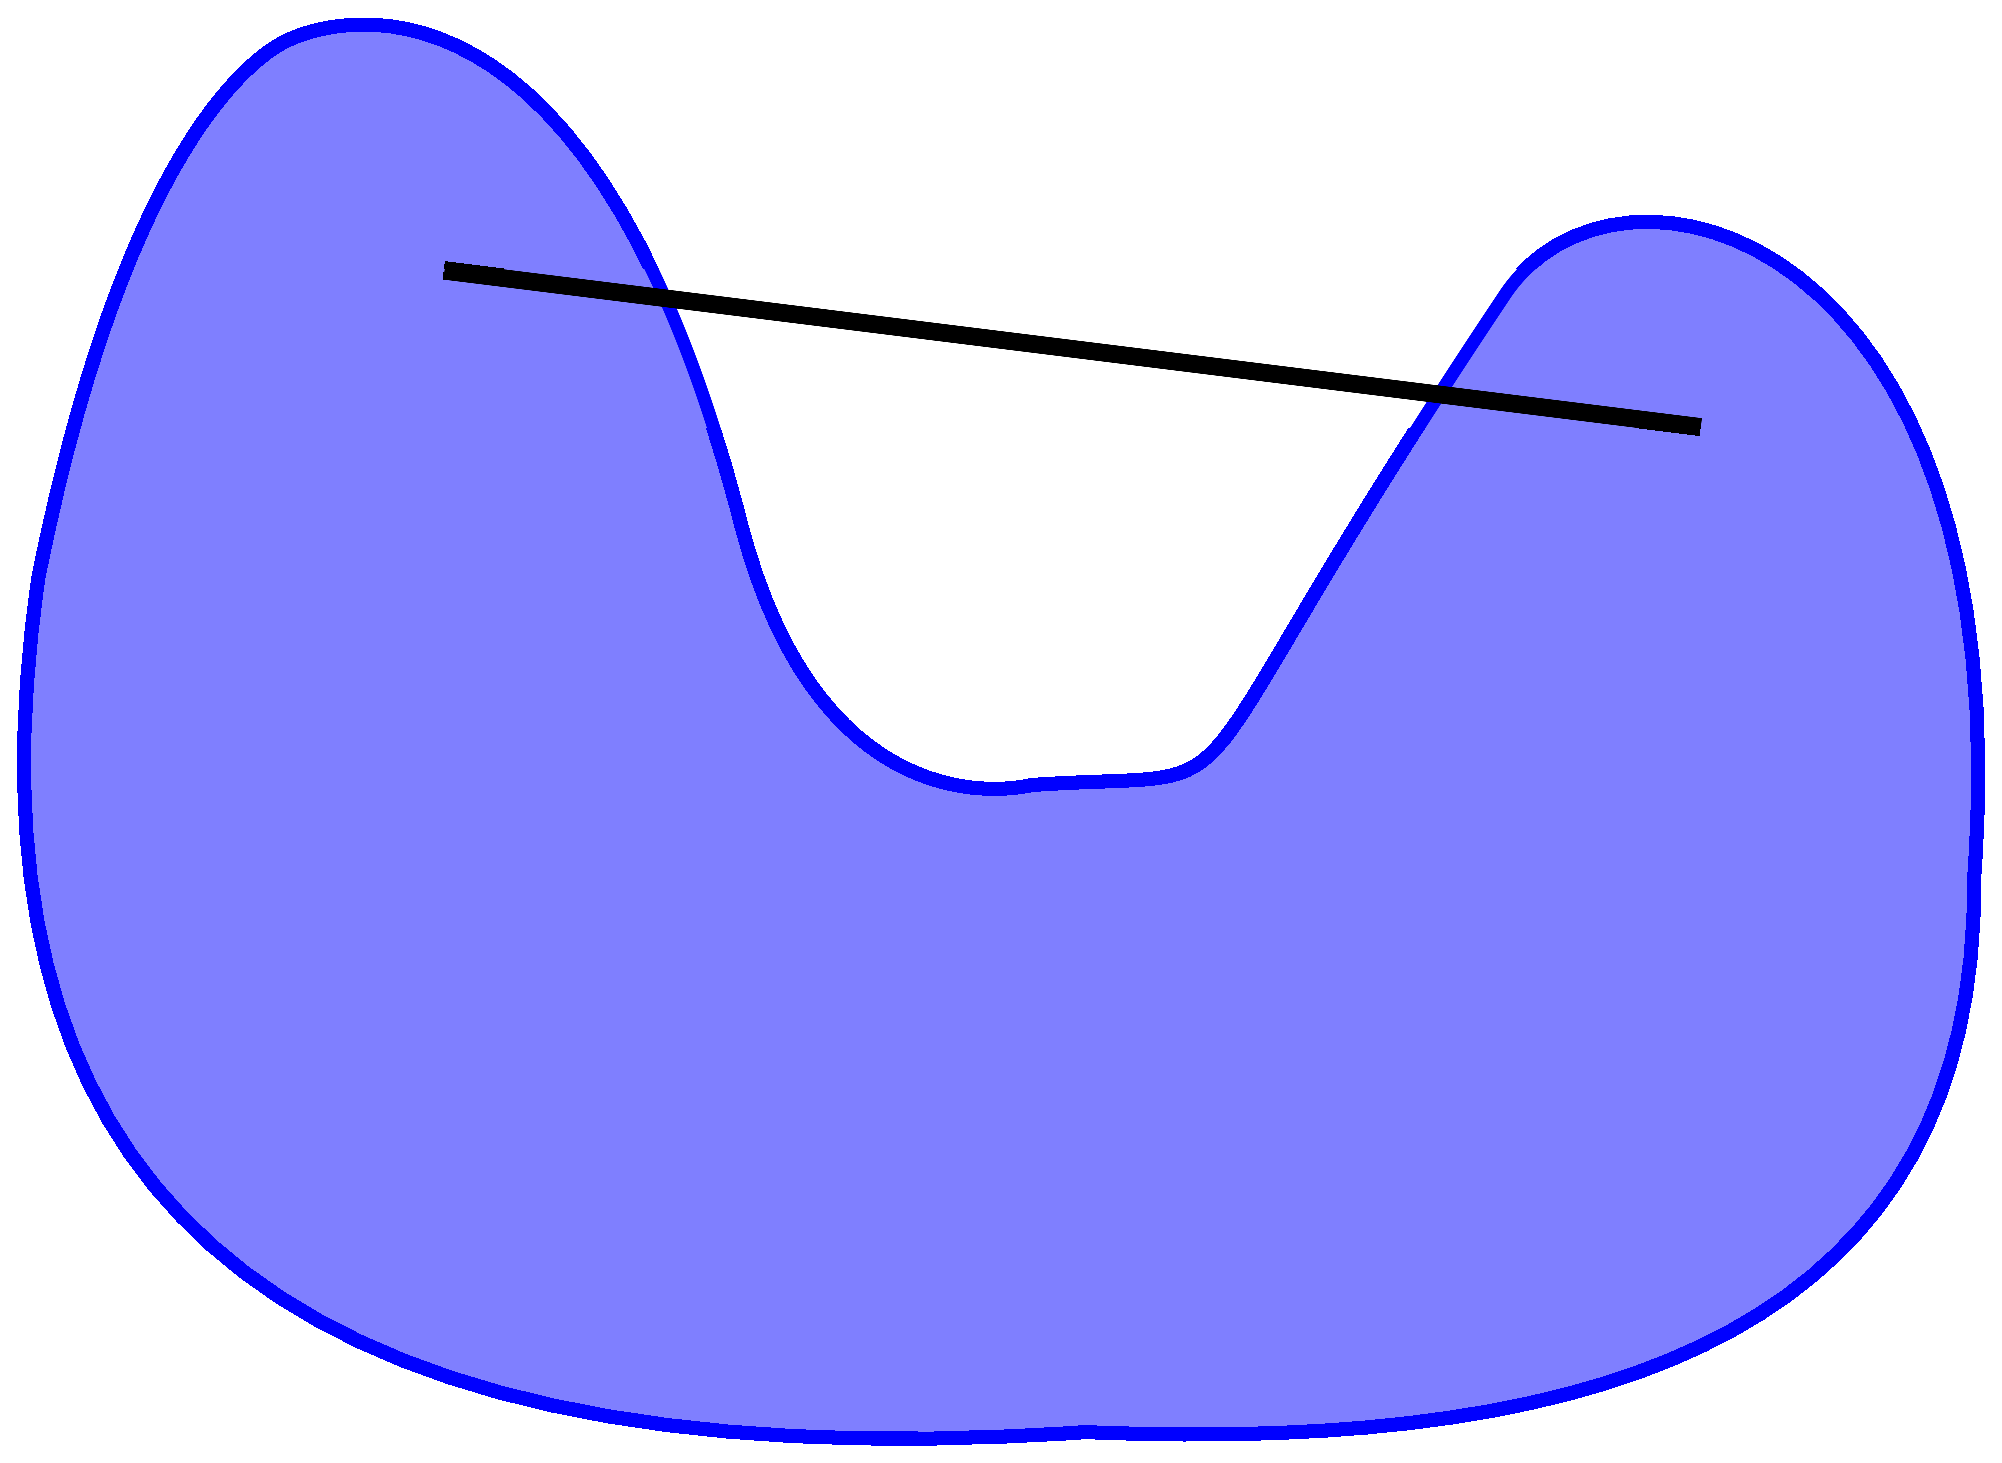
\includegraphics[keepaspectratio, scale=0.095]{figures/eps/non_convex_set.eps}
      \caption{非凸集合}
    \end{minipage}
  \end{figure}
\end{frame}

\begin{frame}{集合最適化}
  数理最適化は1950年以降に急速に発展してきた分野の一つであり、また、2000年以降には機械学習やデータ解析などの応用分野においても広く利用されている。
  現在は、制御理論やゲーム理論に応用される集合最適化の研究を進めている。
  \begin{figure}
    \centering
    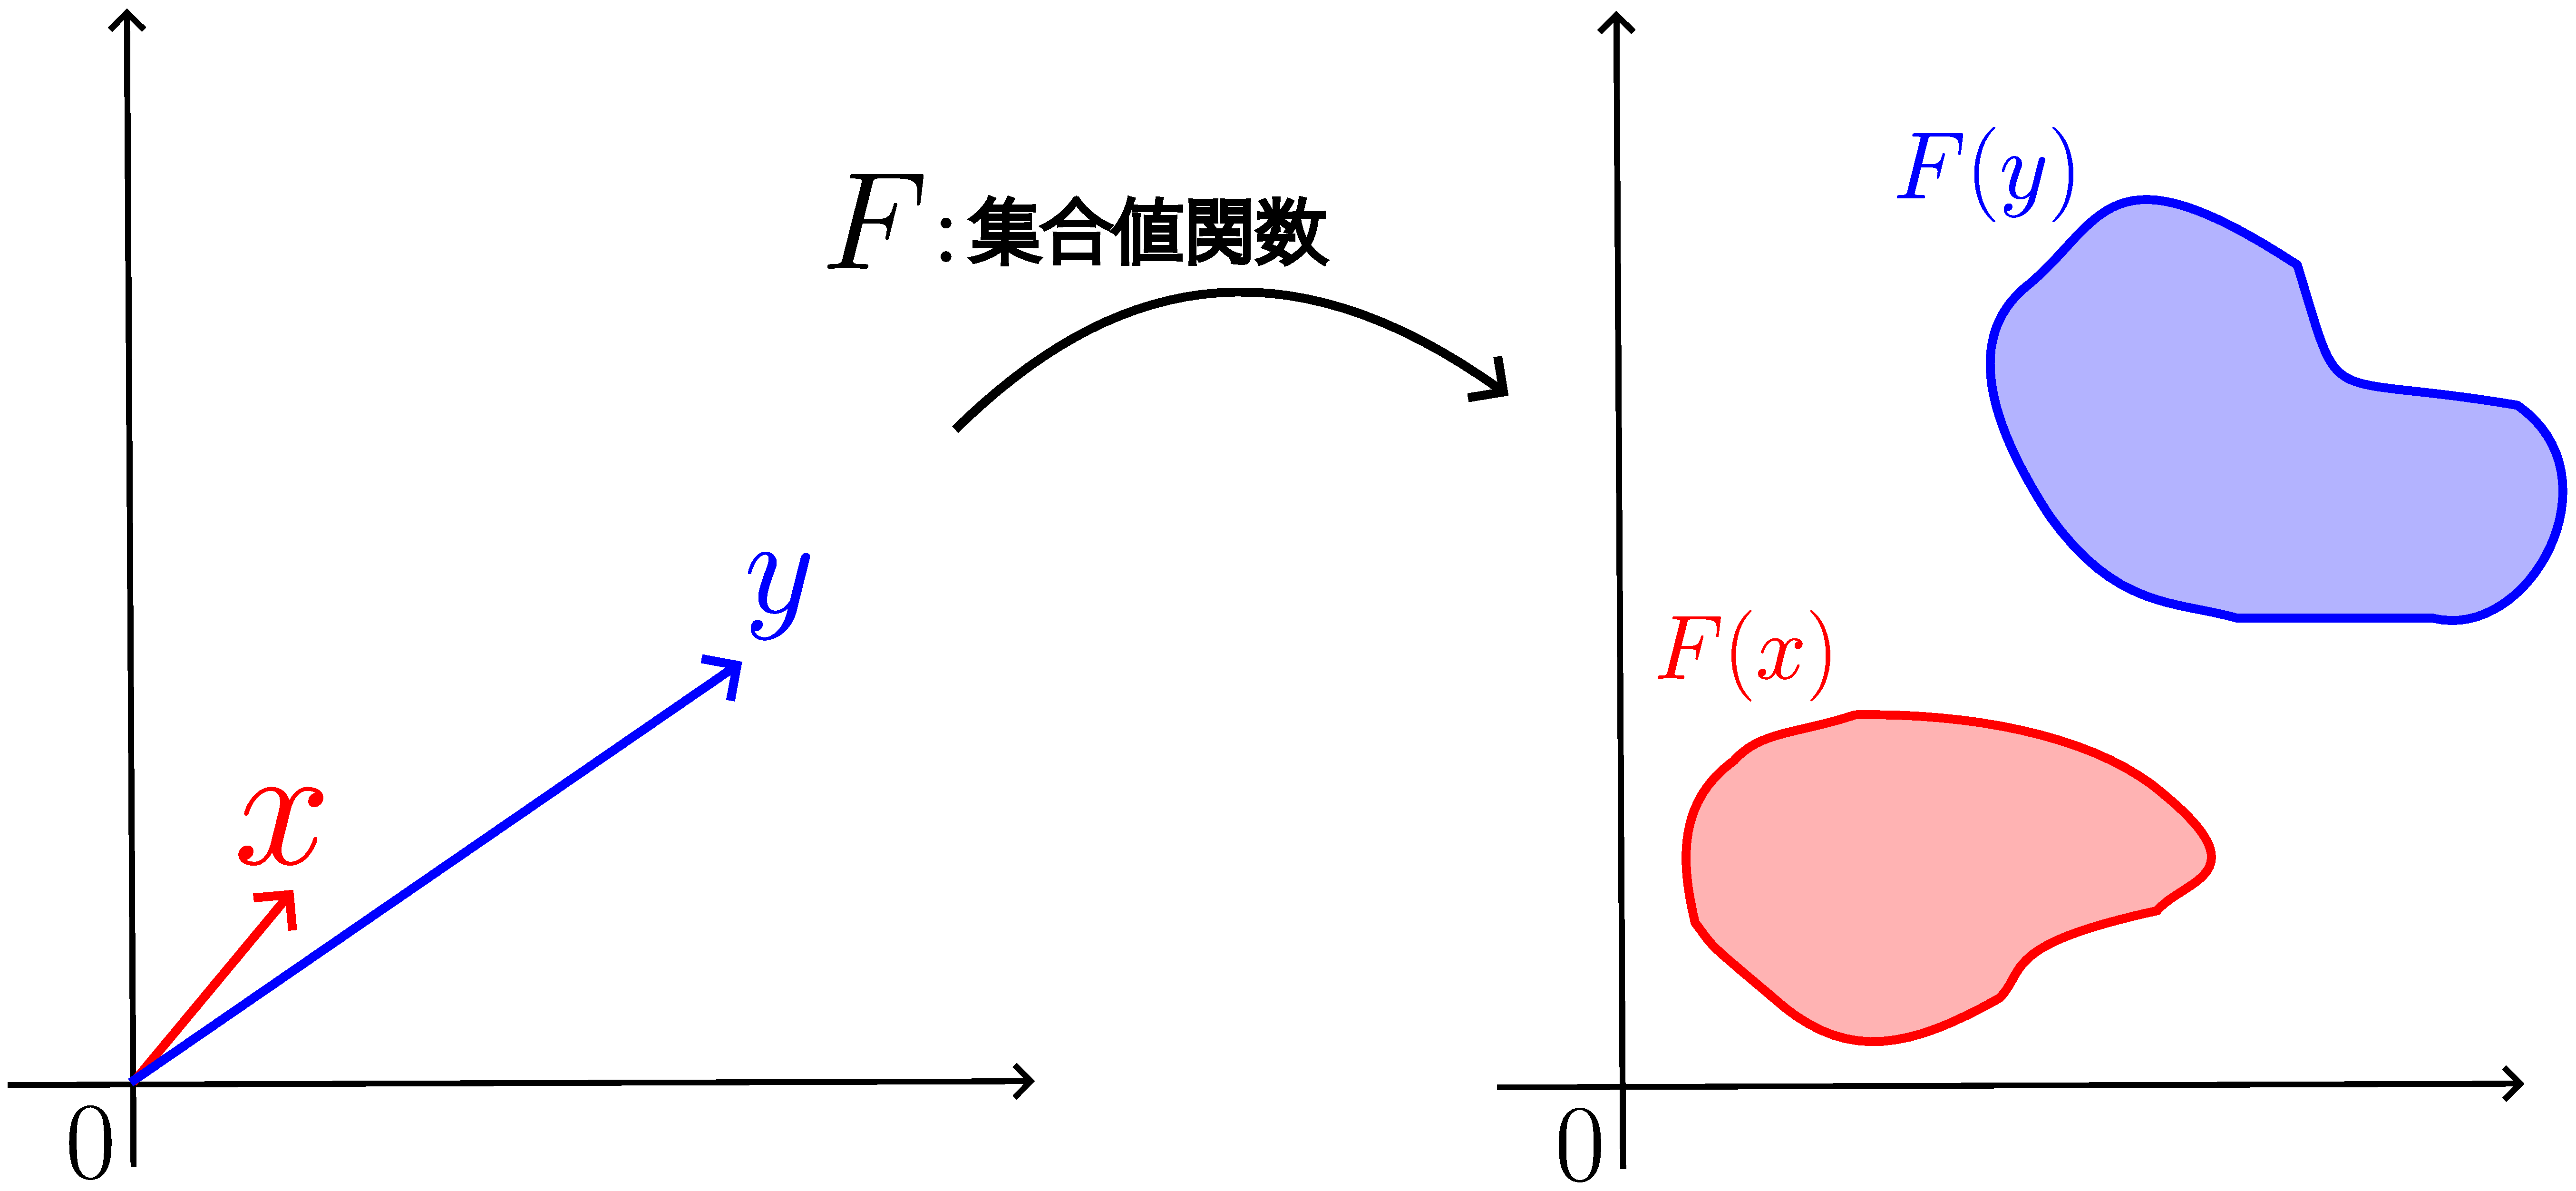
\includegraphics[keepaspectratio, scale=0.10]{figures/eps/set_opt.eps}
    \caption{集合最適化}
  \end{figure}
\end{frame}

\end{document}